\documentclass[a4paper,12pt]{jarticle}
\input ./chap01_preamble.tex
\graphicspath{%
  {../text01-img/}%
}
% !TEX root = ./chap01_04.tex
\begin{document}
\section{HTML(\ruby{自己}{じこ}\ruby{紹介}{しょうかい}のホームページ)}
みなさんがブラウザでけんさくしてホームページを\ruby{表示}{ひょうじ}させました。ホームページはHTML(エイチ ティー エム エル)という言語で書かれています。ブラウザがこれ\ruby{理解}{りかい}して\ruby{表示}{ひょうじ}をしてくれています。HTMLはテキストエディタで\ruby{編集}{へんしゅう}します。ホームページはかんたんに作ることができます。この章では、みなさんも作り方を学び、自分の\ruby{自己}{じこ}\ruby{紹介}{しょうかい}のホームページを作ります。


\bigskip


\bigskip


\bigskip


\bigskip



\begin{figure}[hb]
  \centering
  \begin{minipage}{15.801cm}
    {\upshape
      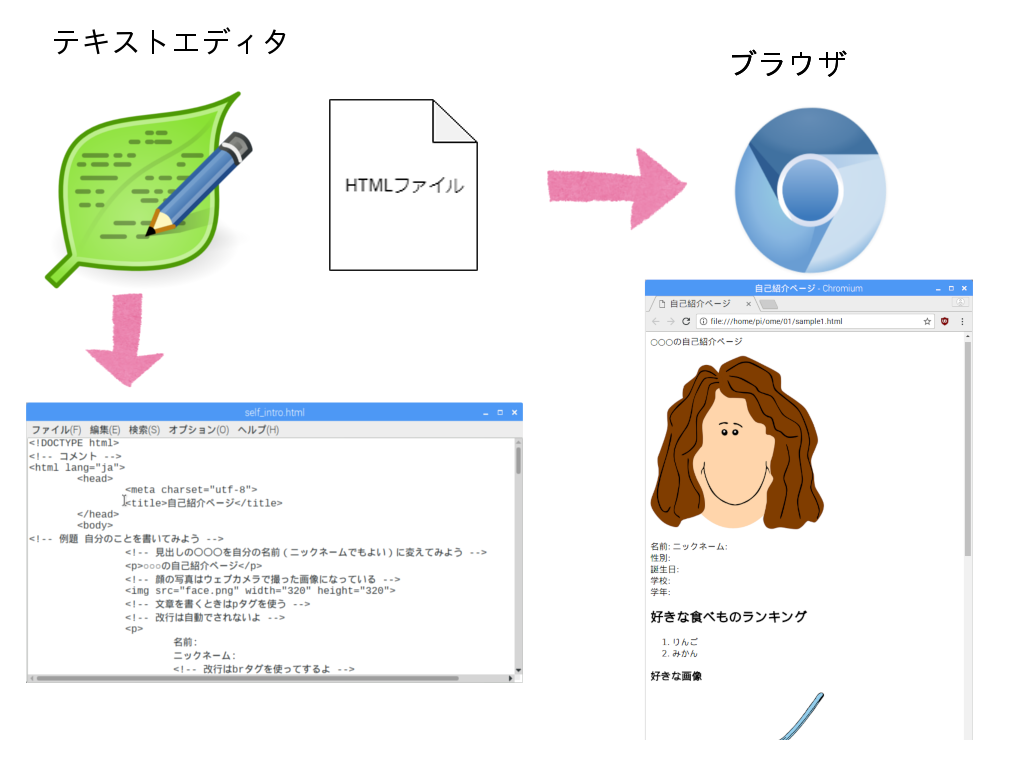
\includegraphics[width=15.801cm]{textbook-img140.png}
      \newline
      \stepcounter{Figure}{\theFigure}: ホームページ作成全体図}
  \end{minipage}
\end{figure}
\clearpage

\begin{figure}
\refstepcounter{Exercise}
\subsection{\theExercise 教材をじぶんのフォルダに置こう}
ホームページの作り方を学ぶための教材は、/usr/local/share/omeというフォルダに置いてあります。
これを、じぶんのフォルダにコピーしましょう。

\textbf{考え方}

  \bigskip

  \centering
  \begin{minipage}{\textwidth}
    \begin{minipage}{0.45\linewidth}
      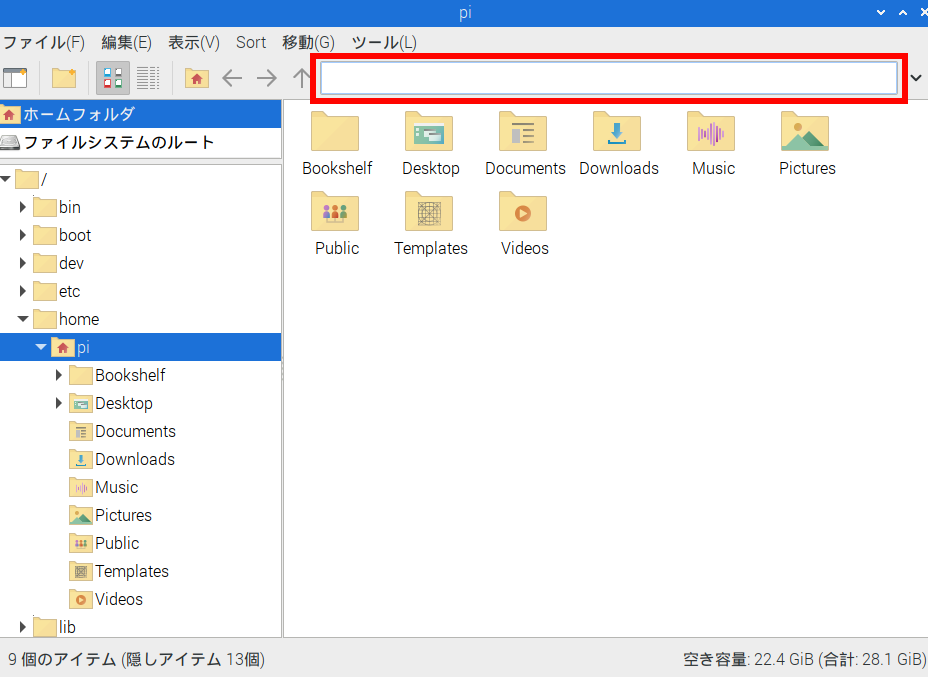
\includegraphics[height=5cm]{textbook-img1010.png}\\
      1.赤い\ruby{枠}{わく}で囲ったところをクリックして、/usr/local/share/omeと入力して、エンターキーを\ruby{押}{お}そう
    \end{minipage}
    \hfill
    \vspace{20pt}
    \begin{minipage}{0.45\linewidth}
      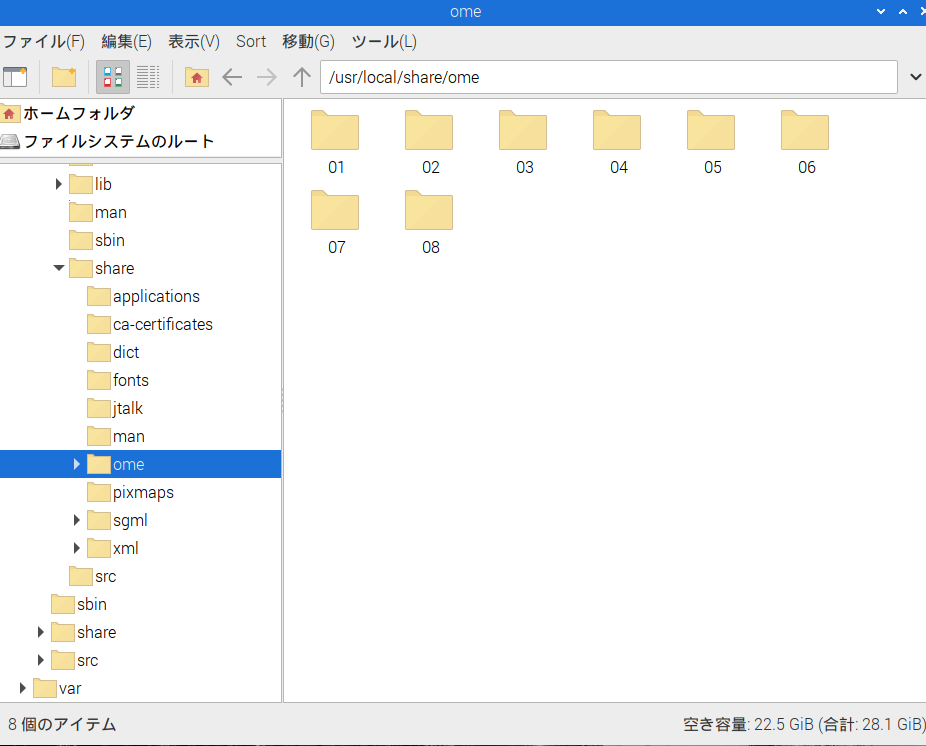
\includegraphics[height=5cm]{textbook-img1011.png}\\
      2.「01」から「08」までのフォルダが\ruby{表示}{ひょうじ}されていることを\ruby{確認}{かくにん}しよう
    \end{minipage}
    \begin{minipage}{0.45\linewidth}
      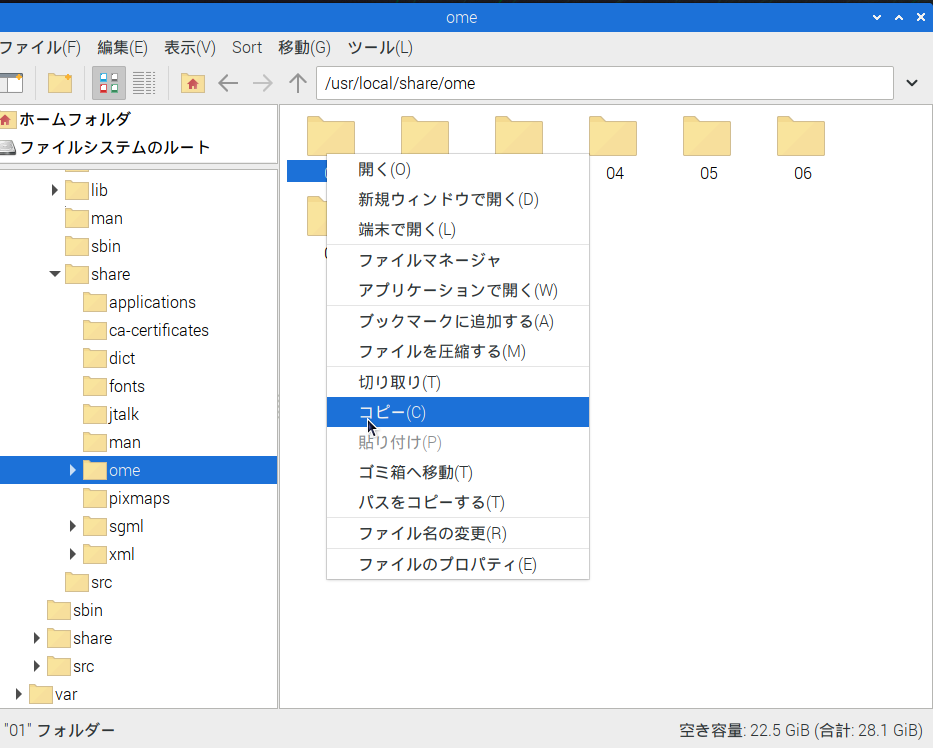
\includegraphics[height=5cm]{textbook-img1012.png}\\
      3.「01」フォルダの上で右クリックし、「コピー」しよう
    \end{minipage}
    \hfill
    \vspace{20pt}
    \begin{minipage}{0.45\linewidth}
      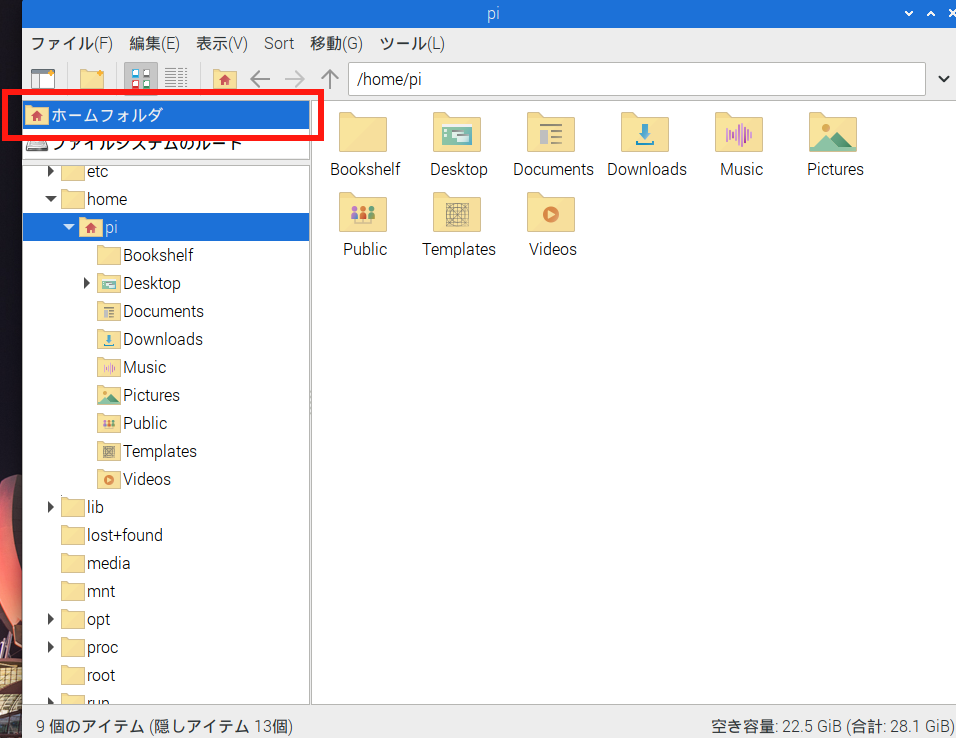
\includegraphics[height=5cm]{textbook-img1013.png}\\
      4.赤い\ruby{枠}{わく}で囲った「ホームフォルダ」をクリックして、自分のフォルダに\ruby{移動}{いどう}しよう
    \end{minipage}    \begin{minipage}{0.45\linewidth}
      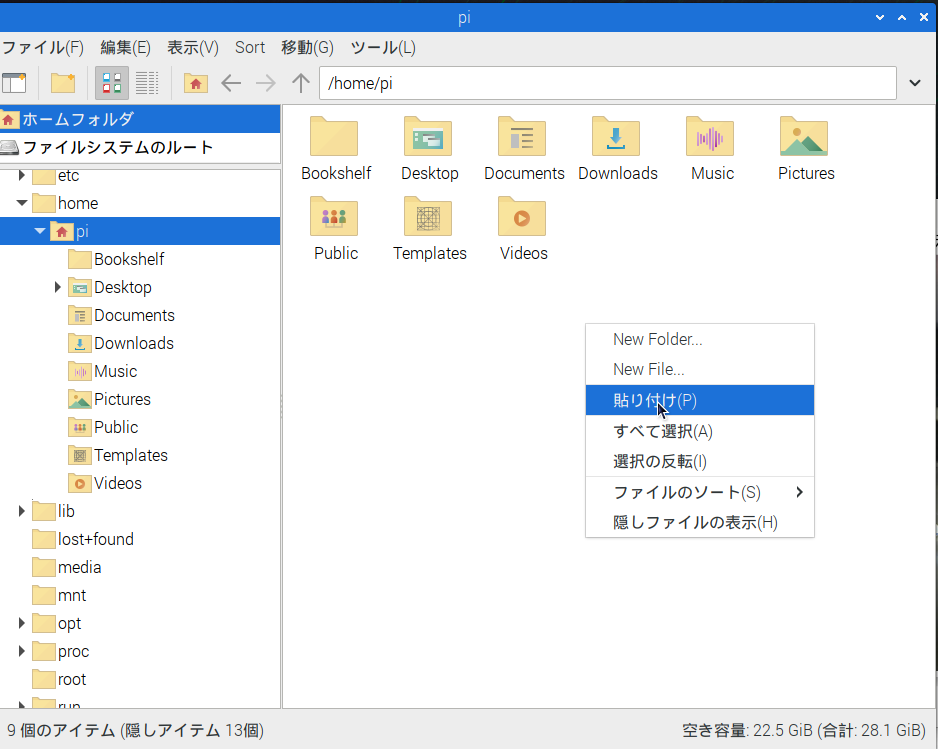
\includegraphics[height=5cm]{textbook-img1014.png}\\
      5.ホームフォルダに\ruby{移動}{いどう}したら、空いているところをクリックして、さっきコピーしたフォルダを「\ruby{貼}{は}り付け」しよう
    \end{minipage}
    \hfill
    \vspace{20pt}
    \begin{minipage}{0.45\linewidth}
      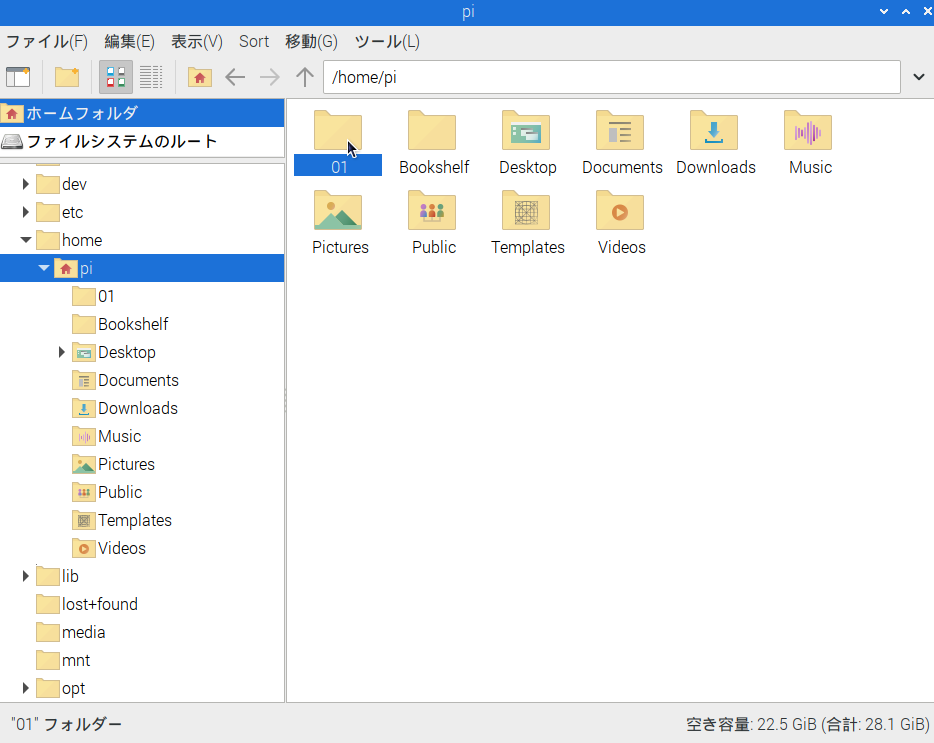
\includegraphics[height=5cm]{textbook-img1015.png}\\
      6.「01」フォルダがあらわれたら、教材のじゅんび\ruby{完了}{かんりょう}だよ
    \end{minipage}

  \end{minipage}

  \bigskip

\end{figure}

\bigskip

\clearpage
\refstepcounter{Exercise}
\subsection{\theExercise ホームページの中身を見てみよう}
\ruby{自己}{じこ}\ruby{紹介}{しょうかい}ページのテンプレートを見てみよう

先ほどコピーした01フォルダにあるself\_intro.htmlをブラウザで開いてみよう

\textbf{考え方}



\begin{figure}[hb]
  \centering
  \begin{minipage}{16.576cm}
    さきほどブラウザでけんさくして見たページを\textbf{ホームページ}(\ruby{正確}{せいかく}にはウェブページ)といいます。ホームページを見るにはブラウザを使用しました。ウェブページはファイル名のあとに.html(エイチ
    ティー エム
    エル)とついています。ブラウザはこのhtmlファイルを見ることが目的です。ファイルをダブルクリックすると自動的にブラウザがhtmlファイルを開いてくれます。\ruby{表示}{ひょうじ}されたホームページを見てみましょう。ファイルマネージャーで01フォルダを開きます。

    赤わくで囲われたところが

    /home\textbf{/自分のユーザ名/01}

    なっていることを\ruby{確認}{かくにん}しておきましょう(この\ruby{画像}{がぞう}の場合だと、ユーザ名がpiなので、/home/pi/01になるよ)

    その中にあるself\_intro.html(黒わくのファイル)をダブルクリックして開きます。




    \bigskip
  \end{minipage}

  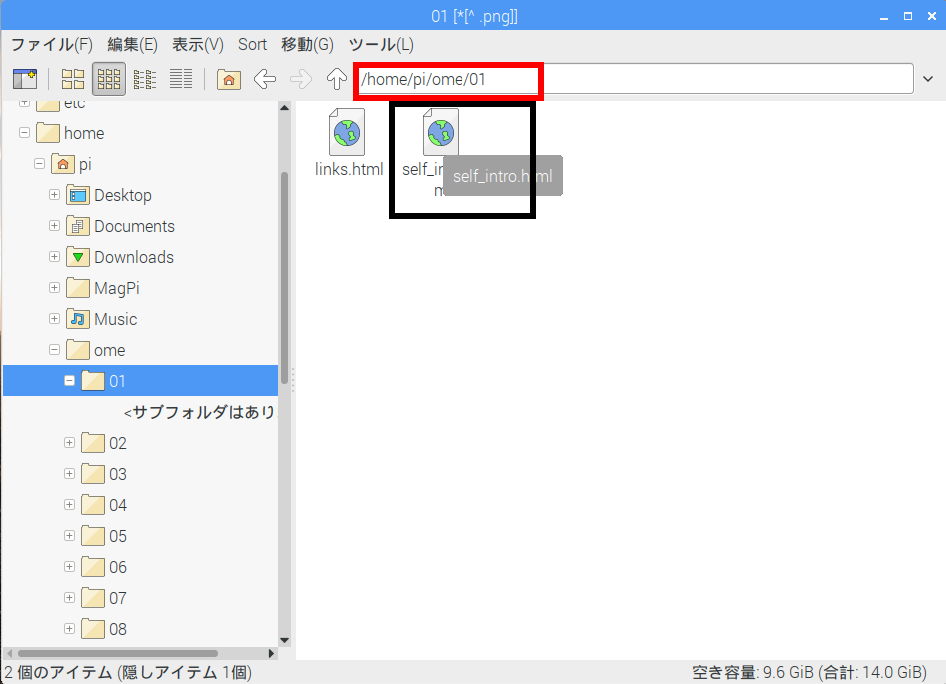
\includegraphics[width=0.8\textwidth]{textbook-img141.png}

\end{figure}

\bigskip

\clearpage
\textbf{答え}



\begin{figure}[hb]
  \centering
  \begin{minipage}{\textwidth}
    このようにホームページが\ruby{表示}{ひょうじ}されればOKです。

    \centering
    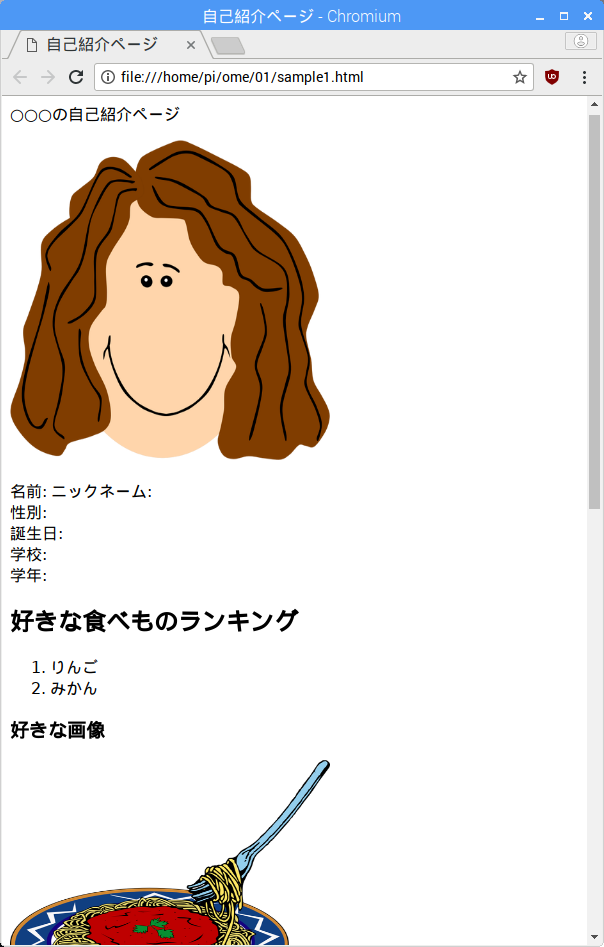
\includegraphics[width=\textwidth]{textbook-img142.png}
  \end{minipage}

\end{figure}
\refstepcounter{Question}\theQuestion\label{Q:hasAnswer04-1}

01フォルダを開いて、links.htmlをブラウザで開いてみよう


\bigskip

\vfill

\clearpage
\begin{figure}[ht]
  \refstepcounter{Exercise}
  \subsection{\theExercise ホームページの中身をのぞいてみよう}
  \addtocounter{Exercise}{-1}\refstepcounter{Exercise}\label{E:HTML_1}
  self\_intro.htmlをテキストエディタで開いて~\ref{seq:refFigure31}のタイトルバーの文字を\ruby{変更}{へんこう}してみよう。タイトルバーは~\ref{seq:refFigure31}のように赤わくで囲われています。


  \bigskip



  \centering
  \begin{minipage}{\textwidth}
    {\upshape
      %\newline
      {\refstepcounter{Figure}\theFigure\label{seq:refFigure31}}:
      ブラウザタイトルバー}
  \end{minipage}

  \centering
  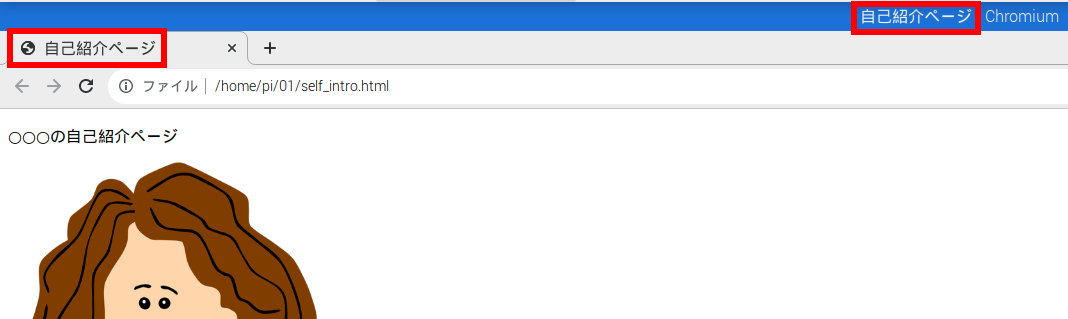
\includegraphics[width=\textwidth]{textbook-img143.png}
  \flushleft
  \textbf{考え方}

  \begin{minipage}{\textwidth}
    \flushleft
    まずは、Text
    Editorでself\_intro.htmlを開いてみましょう。
    \begin{minipage}{0.45\linewidth}
      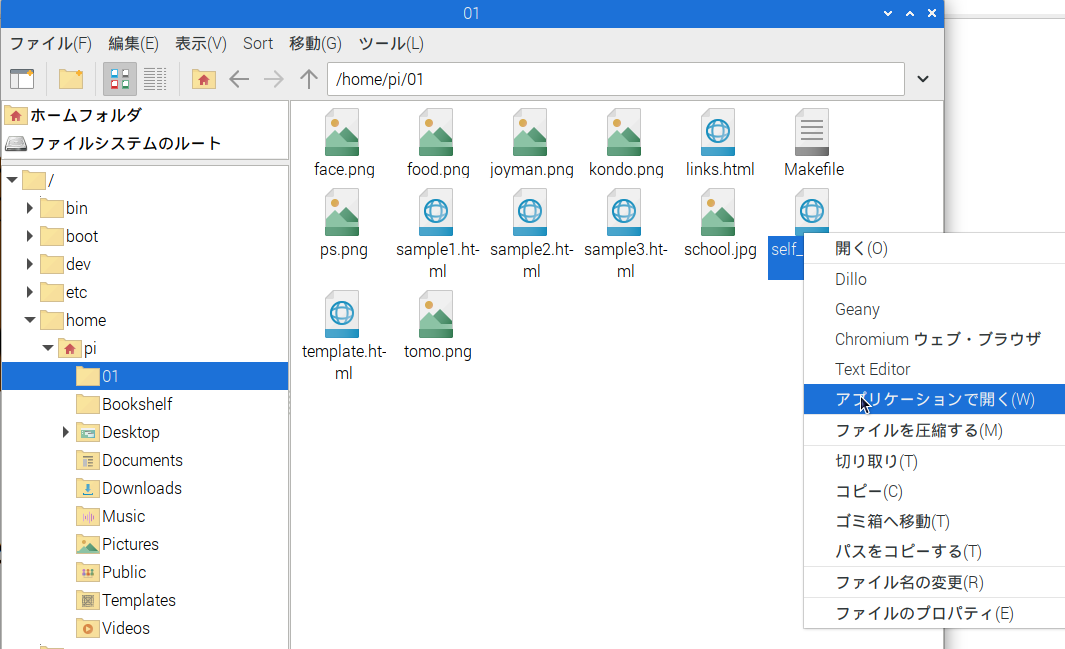
\includegraphics[width=\linewidth]{textbook-img1040.png}\\
      1.self\_intro.htmlを右クリックして、「アプリケーションで開く」をクリックします。
    \end{minipage}
    \hfill
    \vspace{20pt}
    \begin{minipage}{0.45\linewidth}
      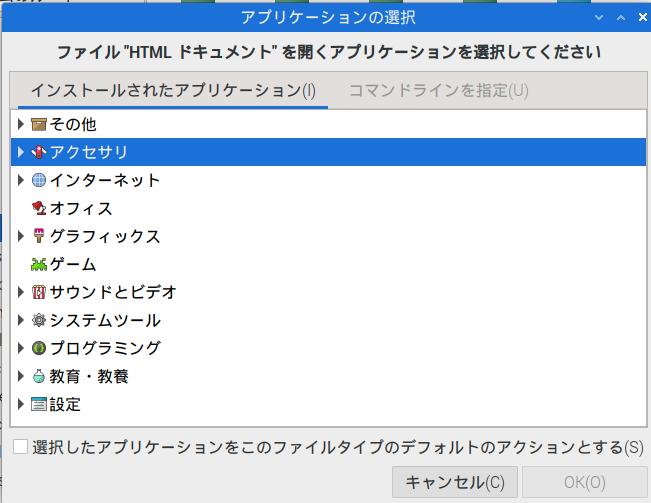
\includegraphics[width=\linewidth]{textbook-img1041.png}\\
      2.「アプリケーションの\ruby{選択}{せんたく}」ウィンドウがでるので、「アクセサリ」をダブルクリックします。
    \end{minipage}
    \begin{minipage}{0.45\linewidth}
      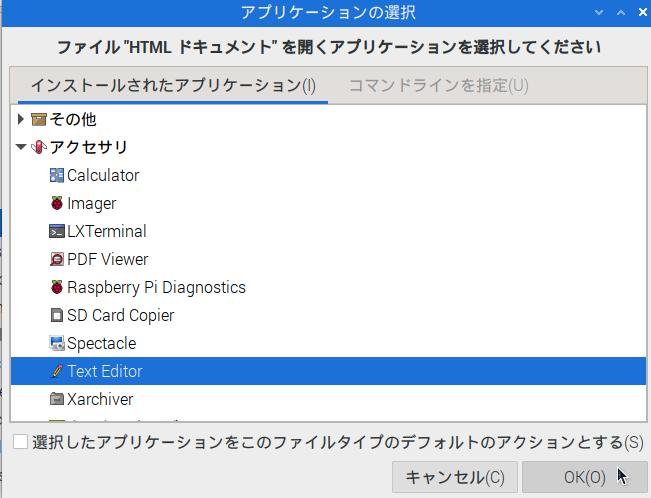
\includegraphics[width=\linewidth]{textbook-img1042.png}\\
      3.「Text Editor」を選んで、OKをクリックします。
    \end{minipage}
  \end{minipage}


\end{figure}

\clearpage
\textbf{考え方(続き)}

Text Editorで開いたら赤線が引かれた
{\textless}title{\textgreater}\textbf{\ruby{自己}{じこ}\ruby{紹介}{しょうかい}ページ}{\textless}/title{\textgreater}
を見てみましょう。\textbf{\ruby{自己}{じこ}\ruby{紹介}{しょうかい}ページ}を\ruby{変更}{へんこう}してみましょう。
この例では\textbf{青梅太郎の\ruby{自己}{じこ}\ruby{紹介}{しょうかい}ページ}と\ruby{変更}{へんこう}します。青梅太郎は自分の名前に置き\ruby{換}{か}えてください。


\centering
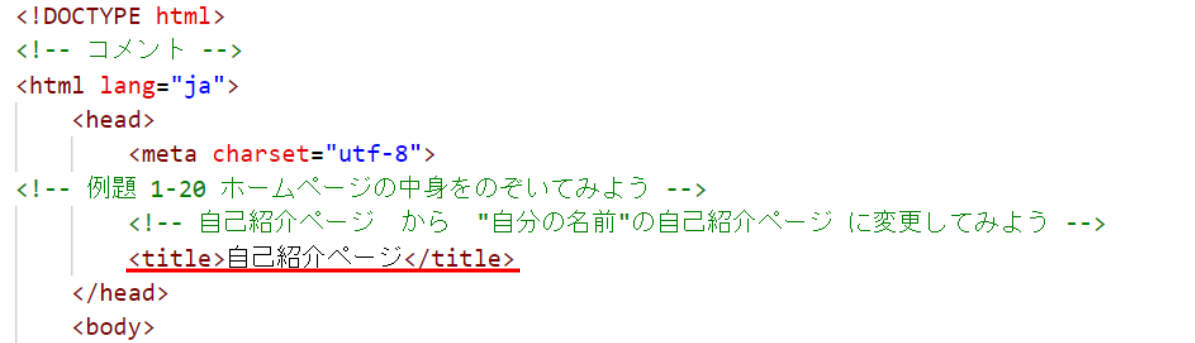
\includegraphics[width=0.9\textwidth]{textbook-img146.png}



\bigskip

\flushleft
\ruby{変更}{へんこう}した例です。

\centering
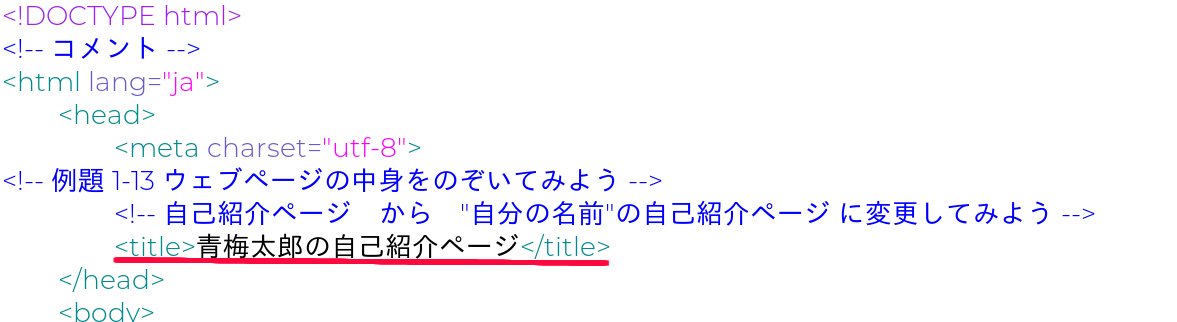
\includegraphics[width=0.9\textwidth]{textbook-img148.png}


\bigskip

\flushleft
\ruby{変更}{へんこう}ができたら、ファイルを\ruby{保存}{ほぞん}します。もう一度ファイルの\ruby{保存}{ほぞん}の手順を\ruby{確認}{かくにん}しておきます。

ファイルー>\ruby{保存}{ほぞん}でファイルを\ruby{保存}{ほぞん}することができます。



\centering
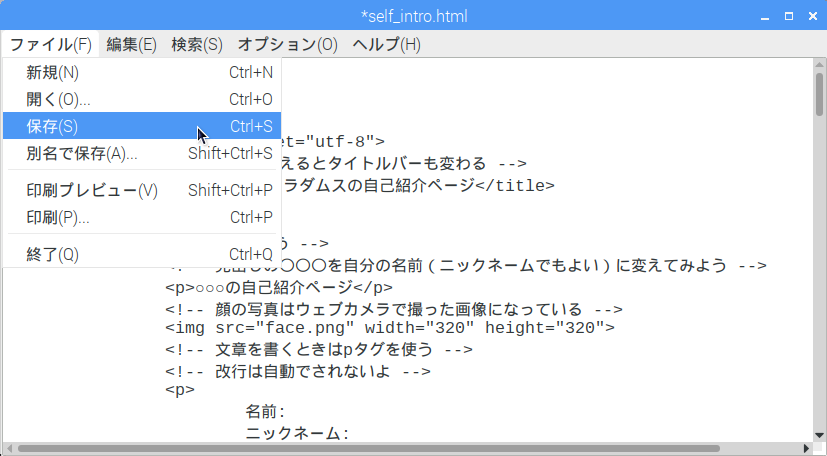
\includegraphics[width=0.8\textwidth]{textbook-img147.png}



\clearpage
\flushleft
\textbf{考え方(続き)}




ファイルに\ruby{変更}{へんこう}をして\ruby{保存}{ほぞん}をしました。
\ruby{変更}{へんこう}を見るためには、ブラウザで新しく\ruby{保存}{ほぞん}したファイルを読み直す必要があります。
ブラウザでページを読み直すことをリロードといいます。


\bigskip


\bigskip
\centering
%[Warning: Image ignored] % Unhandled or unsupported graphics:
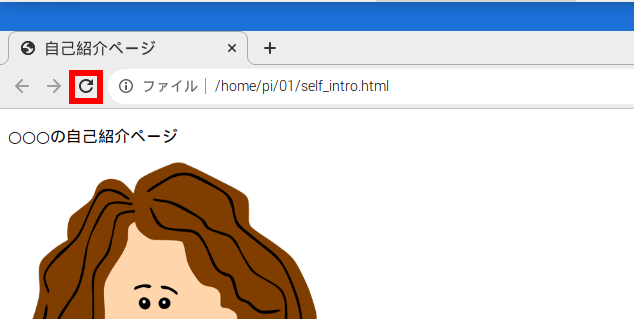
\includegraphics[width=0.8\textwidth]{textbook-img149.png}

\flushleft
赤わくで囲われたように、円の形をした矢印があります。これをクリックすることでリロードができます。これで、\ruby{変更}{へんこう}結果がブラウザへ\ruby{反映}{はんえい}されます。

\vfill
\clearpage
\textbf{答え}


{\textless}title{\textgreater}\textbf{青梅太郎の\ruby{自己}{じこ}\ruby{紹介}{しょうかい}ページ}{\textless}/title{\textgreater}\\
と\ruby{変更}{へんこう}をしたのでブラウザのタイトルバー(赤わくで囲われた部分)はこれに\ruby{対応}{たいおう}して\textbf{青梅太郎の\ruby{自己}{じこ}\ruby{紹介}{しょうかい}ページ}と変わっていますね。

\ruby{皆}{みな}さんは、自分の名前が\ruby{表示}{ひょうじ}されていると思います。

\centering
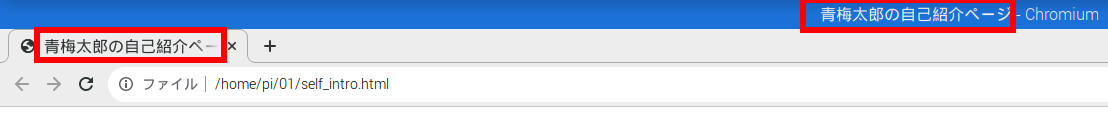
\includegraphics[width=0.85\textwidth]{textbook-img152.png}
\flushleft


二行目に注目してください。

\centering
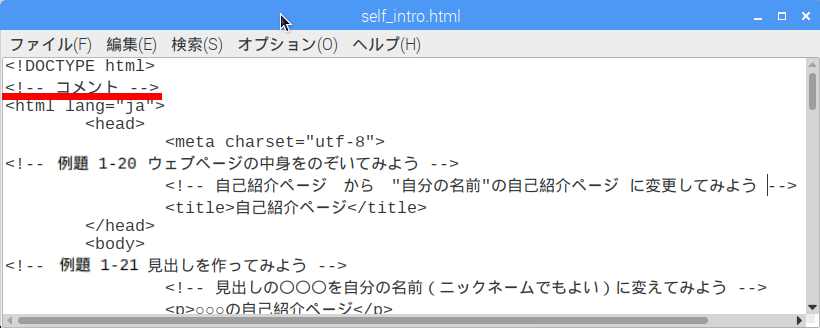
\includegraphics[width=0.85\textwidth]{textbook-img151.png}
\flushleft



\bigskip

{\textless}!- -コメント -
-{\textgreater} という行があります。

これをコメントよびます。囲われたものはブラウザには\ruby{表示}{ひょうじ}されません。

コメントはメモとして使えます。はじめの{\textless}!-{}-と終わりの{}-{}-{\textgreater}にはスペースは入れてはいけません。この記号の間であれば改行をしても\ruby{構}{かま}いません。試しにメモを追加してみましょう。

変えた行の上に

\textbf{ここを変えるとタイトルバーも変わる
}

と追加しましょう。このファイルにはコメントがたくさん書いてあります。\ruby{変更}{へんこう}する前に読んでみてください。コメントはなるべく書いてわかりやすくしておきましょう。


\centering
%[Warning: Image ignored] % Unhandled or unsupported graphics:
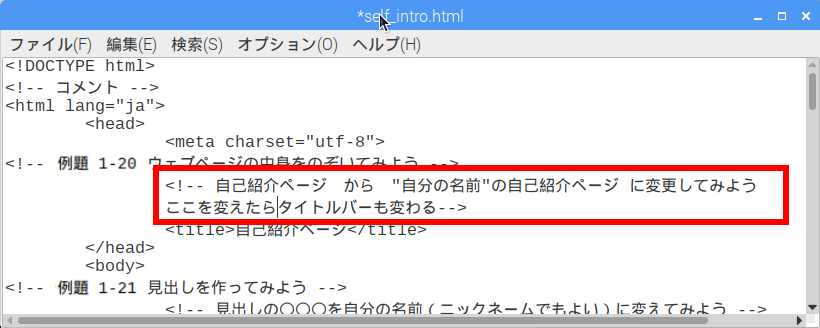
\includegraphics[width=0.85\textwidth]{textbook-img150.png}


\vfill
\clearpage
\begin{figure}[ht]
  \refstepcounter{Exercise}
  \subsection{\theExercise 見出しを作ってみよう}
  \addtocounter{Exercise}{-1}\refstepcounter{Exercise}\label{E:HTML_2}


  \centering
  \begin{minipage}{\textwidth}
    {\upshape
      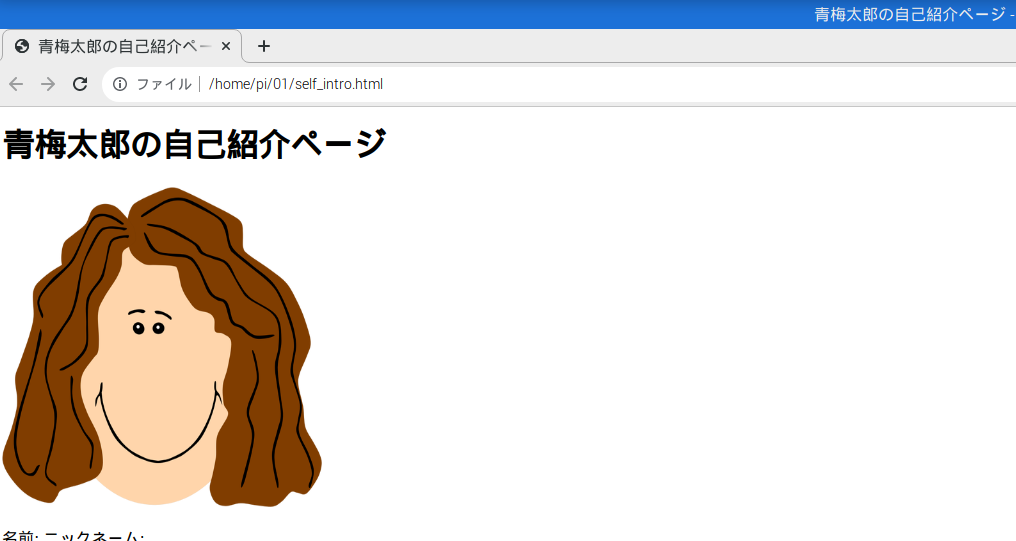
\includegraphics[width=0.7\textwidth]{textbook-img153.png}
      \newline
      \stepcounter{Figure}{\theFigure}: 見出しをつくってみよう}
  \end{minipage}


  \bigskip
  \flushleft

  \textbf{考え方}



  \begin{minipage}{\textwidth}
    \flushleft

    HTMLだけでなく見出しを作ることは読みやすい文書を作成するのに重要です。また、改行を\ruby{適切}{てきせつ}に行うことも大切です。

    まずは、見出しを作ってみましょう。\textbf{〇〇〇の\ruby{自己}{じこ}\ruby{紹介}{しょうかい}ページ}を\ruby{変更}{へんこう}してみよう


    \bigskip

    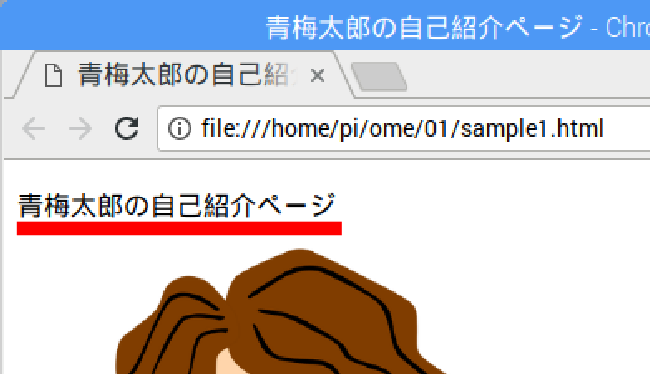
\includegraphics[width=0.7\textwidth]{textbook-img154.png}


    \bigskip

    テキストエディタで\ruby{変更}{へんこう}してみよう。\ruby{変更}{へんこう}したら\ruby{保存}{ほぞん}してブラウザをリロードするのを忘れないようにしよう。


    \bigskip

    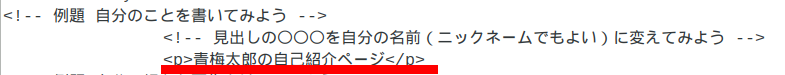
\includegraphics[width=0.9\textwidth]{textbook-img155.png}


    \bigskip


    見出しとしてはまだ文字が小さく目立たないですね。もっと大きくしてみましょう。




    \bigskip
  \end{minipage}

\end{figure}

\clearpage
\flushleft
\textbf{考え方(続き)}




次の行

{\textless}p{\textgreater}青梅太郎の\ruby{自己}{じこ}\ruby{紹介}{しょうかい}ページ{\textless}/p{\textgreater}

\bigskip

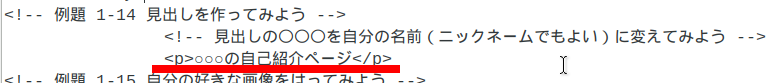
\includegraphics[width=0.9\textwidth]{textbook-img158.png}

から

{\textless}h1{\textgreater}青梅太郎の\ruby{自己}{じこ}\ruby{紹介}{しょうかい}ページ{\textless}/h1{\textgreater}

に変えてみましょう。\ruby{保存}{ほぞん}してブラウザをリロードしてみてください。


\bigskip

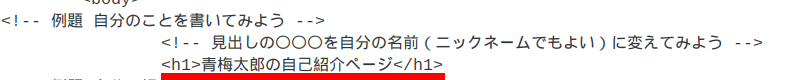
\includegraphics[width=0.9\textwidth]{textbook-img157.png}


\bigskip


\bigskip

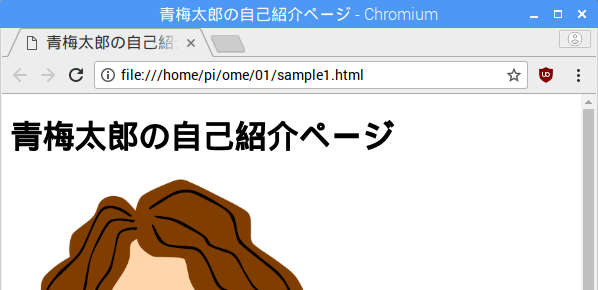
\includegraphics[width=0.4\textwidth]{textbook-img156.png}


今度は見出しらしく太文字で目立つようにになりましたね。




\bigskip

{\textless}p{\textgreater}青梅太郎の\ruby{自己}{じこ}\ruby{紹介}{しょうかい}ページ{\textless}/p{\textgreater} から

{\textless}h1{\textgreater}青梅太郎の\ruby{自己}{じこ}\ruby{紹介}{しょうかい}ページ{\textless}/h1{\textgreater} へ\ruby{変更}{へんこう}したら文字が太く大きくなりました。


\bigskip

{\textless}p{\textgreater}文字{\textless}/p{\textgreater}や{\textless}h1{\textgreater}文字{\textless}/h1{\textgreater}のようなものをそれぞれpタグ、h1タグといいます。\textbf{タグ}にはそれぞれ\ruby{役割}{やくわり}があります。タグの間に\ruby{挟}{はさ}まれている文字に\ruby{効果}{こうか}があります。

\begin{itemize}
  \item 文字の前にある{\textless}p{\textgreater}を\textbf{開始タグ}
  \item 文字の後にある{\textless}/p{\textgreater}を\textbf{\ruby{終了}{しゅうりょう}タグ}
\end{itemize}

\textbf{タグには半角文字しかつかえません。}

\begin{itemize}
  \item pタグは、文章として\ruby{表示}{ひょうじ}をします。文章を書くときに使用します。

  \item h1タグは見出しとして\ruby{表示}{ひょうじ}をします。見出しを作るときに使用します。
\end{itemize}


\vfill

\refstepcounter{Question}\theQuestion\label{Q:hasAnswer04-2}

\begin{itemize}
  \item[]
    h1をh2、h3、h4、h5、h6にそれぞれ変えてみてどうなるか確かめてみましょう。
\end{itemize}

\bigskip

\clearpage\subsection{\ruby{授業}{じゅぎょう}で使用するタグのいちらん}
{\small
  \begin{center}
    \tablefirsthead{}
    \tablehead{}
    \tabletail{}
    \tablelasttail{}
    \begin{supertabular}{|m{1.6cm}|m{5.1060004cm}|m{7.8930006cm}|m{2.037cm}|}
      \hline
      タグ名 &
      使用例 &
      \ruby{効果}{こうか} &
      例題番号\\\hline
      title &
      {\textless}title{\textgreater}タイトル{\textless}/title{\textgreater} &
      ブラウザのタイトルバーをタイトルに\ruby{変更}{へんこう}する
      &
      \ref*{E:HTML_1}\\\hline
      p &
      {\textless}p{\textgreater}文章{\textless}/p{\textgreater} &
      文章と\ruby{表示}{ひょうじ}する。改行なし &
      \ref*{E:HTML_2}\\\hline
      h1 &
      {\textless}h1{\textgreater}見出し1{\textless}/h1{\textgreater} &
      見出し1と\ruby{表示}{ひょうじ}する。\ruby{普通}{ふつう}の文字より大きい
      &
      \ref*{E:HTML_2}\\\hline
      img &
      {\textless}img src=”img.png”{\textgreater} &
      src=””で指定された\ruby{画像}{がぞう}ファイルを\ruby{表示}{ひょうじ}する
      &
      \ref*{E:HTML_3}\\\hline
      br &
      {\textless}br{\textgreater} &
      改行をする &
      \ref*{E:HTML_4}\\\hline
      ol &
      {\textless}ol{\textgreater}

      \ \ {\textless}li{\textgreater}1位{\textless}/li{\textgreater}

      {\textless}/ol{\textgreater} &
      liタグと合わせて使用する。\ruby{順序}{じゅんじょ}付きのリストを作る。\ruby{順序}{じゅんじょ}はliタグの順番通りにつく
      &
      \ref*{E:HTML_5}\\\hline
      Ul &
      {\textless}ul{\textgreater}

      \ \ {\textless}li{\textgreater}1位{\textless}/li{\textgreater}

      {\textless}/ul{\textgreater} &
      \ruby{順序}{じゅんじょ}なし。${\bullet}で始まるリストを作成。$
      &
      \ref*{E:HTML_7}\\\hline
      i &
      {\textless}i{\textgreater}イタリック{\textless}/i{\textgreater} &
      \ruby{斜}{なな}めの文字を\ruby{表示}{ひょうじ} &
      \ref*{E:HTML_6}\\\hline
      u &
      {\textless}u{\textgreater}アンダーライン{\textless}/u{\textgreater} &
      下線つきの文字を\ruby{表示}{ひょうじ} &
      \ref*{E:HTML_6}\\\hline
      strong &
      {\textless}strong{\textgreater}

      目立つ文字

      {\textless}/strong{\textgreater} &
      文字を目立たせる &
      \ref*{E:HTML_6}\\\hline
      font  &
      {\textless}font color=”\#019a66”{\textgreater}

      \ \ 色付き文字

      {\textless}/font{\textgreater} &
      color=””で指定した色で文字を\ruby{表示}{ひょうじ}。 &
      \ref*{E:HTML_6}\\\hline
      font &
      {\textless}font size=”1”{\textgreater}

      大きさを変える

      {\textless}/font{\textgreater} &
      size=””で指定した文字の大きさで\ruby{表示}{ひょうじ} &
      \ref*{E:HTML_6}\\\hline
      table &
      {\textless}table{\textgreater}

      ~

      {\textless}/table{\textgreater} &
      表を作成するときに使用する。caption, tr, th,
      tdタグといっしょに使用する。 &
      \ref*{E:HTML_7}\\\hline
      caption &
      {\textless}caption{\textgreater}表題{\textless}/caption{\textgreater} &
      表のタイトルを\ruby{表示}{ひょうじ} &
      \ref*{E:HTML_7}\\\hline
      tr &
      {\textless}tr{\textgreater}{\textless}/tr{\textgreater} &
      表の行を作る。th,
      tdタグといっしょに使用する。 &
      \ref*{E:HTML_7}\\\hline
      th &
      {\textless}th{\textgreater}列のタイトル{\textless}/th{\textgreater} &
      表の列のタイトルを\ruby{表示}{ひょうじ}する &
      \ref*{E:HTML_7}\\\hline
      td &
      {\textless}td{\textgreater}列のデータ{\textless}/td{\textgreater} &
      表の列のデータを\ruby{表示}{ひょうじ} &
      \ref*{E:HTML_7}\\\hline
      a &
      {\textless}a href=”google.com”{\textgreater}

      \ \ google

        {\textless}/a{\textgreater} &
      クリックすると登録していたホームページに\ruby{移動}{いどう}する文字を\ruby{表示}{ひょうじ}
      &
      \ref*{E:HTML_8}\\\hline
    \end{supertabular}
  \end{center}
}

\bigskip
ホームページを作るときには、これらのタグをたくさん使用します。使い方を例題とともに学んでいきましょう。


\clearpage


{\centering\bfseries
  タグは半角文字で入力しなければなりません。
  \par}

{\centering\bfseries
  HTMLファイルでタグを入力する\ruby{際}{さい}は
  \par}

{\centering\bfseries
  \ruby{常}{つね}に右上のアイコンがキーボードになっていることを\ruby{確認}{かくにん}してください。
  \par}

\centering
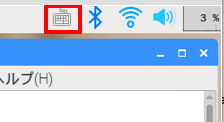
\includegraphics[width=0.6\textwidth]{textbook-img159.png}





\bigskip

\bigskip

\bigskip

\bigskip


{\centering\bfseries
  このアイコンのときは全角入力モードだから
  \par}

\centering
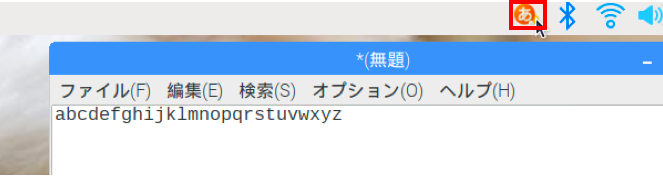
\includegraphics[width=0.6\textwidth]{textbook-img160.png}


\bigskip


\bigskip

{\centering\bfseries
  タグを打つときはCtrl +
  スペースキーを\ruby{押}{お}して半角入力モード
  \par}

{\centering\bfseries
  (キーボードのアイコン)にしよう
  \par}

\clearpage
%\begin{figure}[ht]
\flushleft
\refstepcounter{Exercise}
\subsection{\theExercise 自分の好きな\ruby{画像}{がぞう}をはってみよう}
\addtocounter{Exercise}{-1}\refstepcounter{Exercise}\label{E:embImginHTML}\label{E:HTML_3}
自分のお気に入りの\ruby{画像}{がぞう}を\ruby{紹介}{しょうかい}してみよう。

\centering
\begin{minipage}{6.738cm}
  {\upshape
    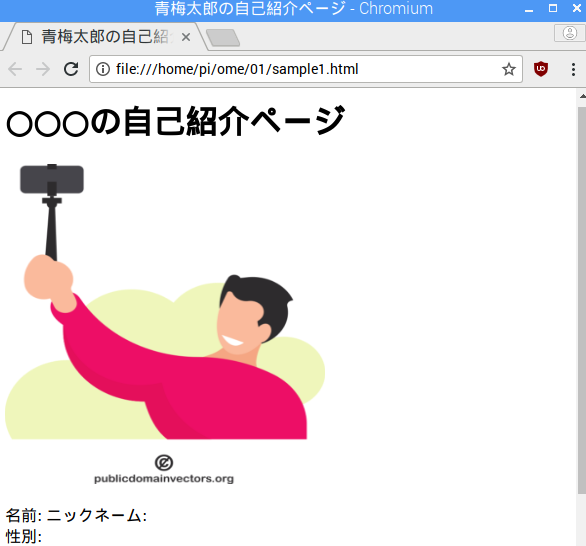
\includegraphics[width=7.071cm,height=6.048cm]{textbook-img161.png}
    \newline
    \stepcounter{Figure}{\theFigure}: 顔写真}
\end{minipage}

\flushleft
\textbf{考え方}


いま、\ruby{髪}{かみ}の長い人の写真が\ruby{表示}{ひょうじ}されているところがあります。このように自分の好きな\ruby{画像}{がぞう}を\ruby{表示}{ひょうじ}させることができます。試しに、ウェブカメラでとった自分の顔に変えてみましょう。

まずは、\ruby{画像}{がぞう}をコピーします。


\bigskip

\begin{minipage}{0.45\linewidth}
  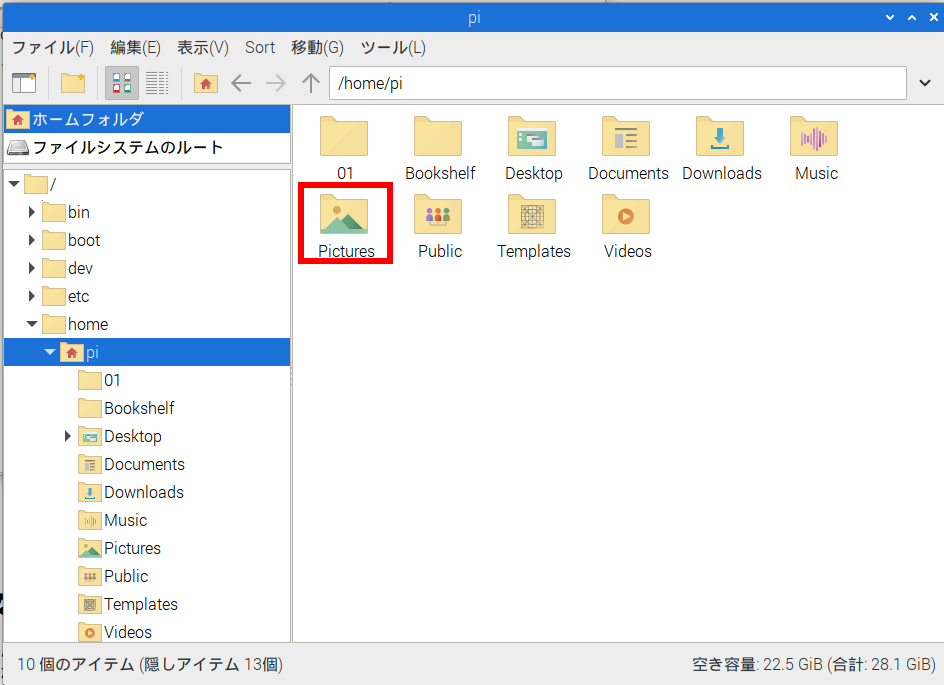
\includegraphics[width=\linewidth]{textbook-img164.png}
  \newline
  1 Picturesをダブルクリック
\end{minipage}
\hspace{10mm}
\begin{minipage}{0.45\linewidth}
  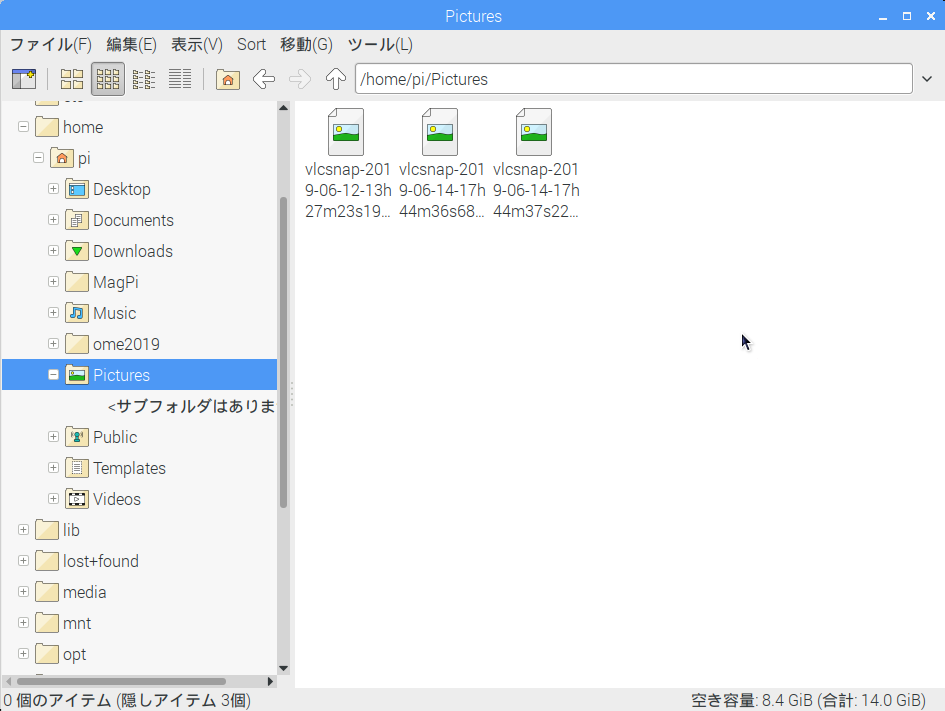
\includegraphics[width=\linewidth]{textbook-img162.png}
  \newline
  2 使いたい\ruby{画像}{がぞう}を右クリック
\end{minipage}

\bigskip

\begin{minipage}{0.45\linewidth}
  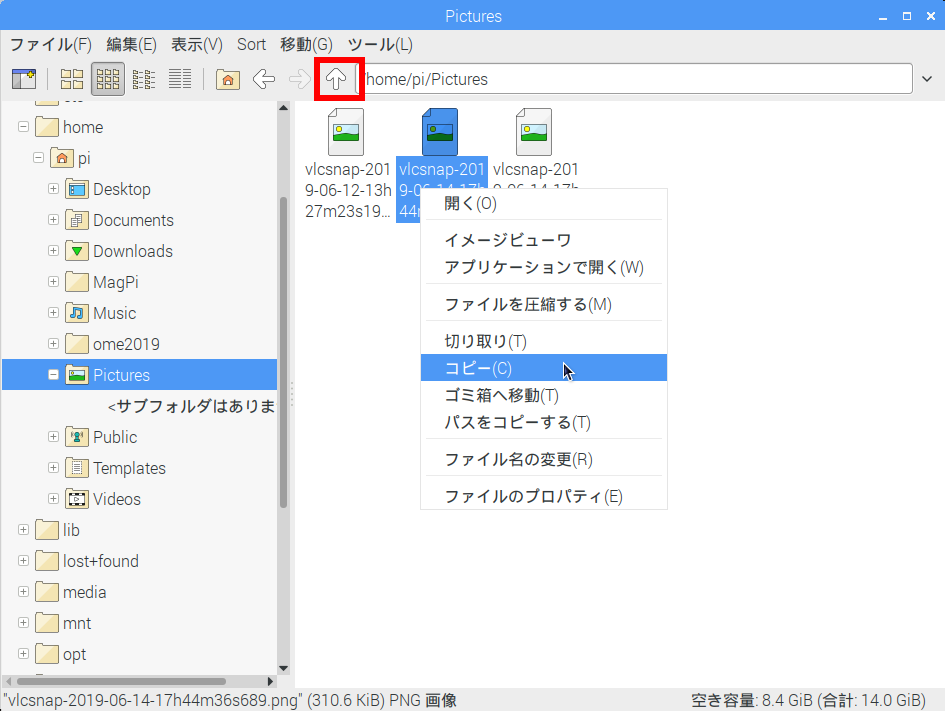
\includegraphics[width=\linewidth]{textbook-img163.png}
  \newline
  3
  コピーを\ruby{選択}{せんたく}・\ruby{赤枠}{あかわく}の上矢印をクリック
\end{minipage}
\hspace{10mm}
\begin{minipage}{0.45\linewidth}
  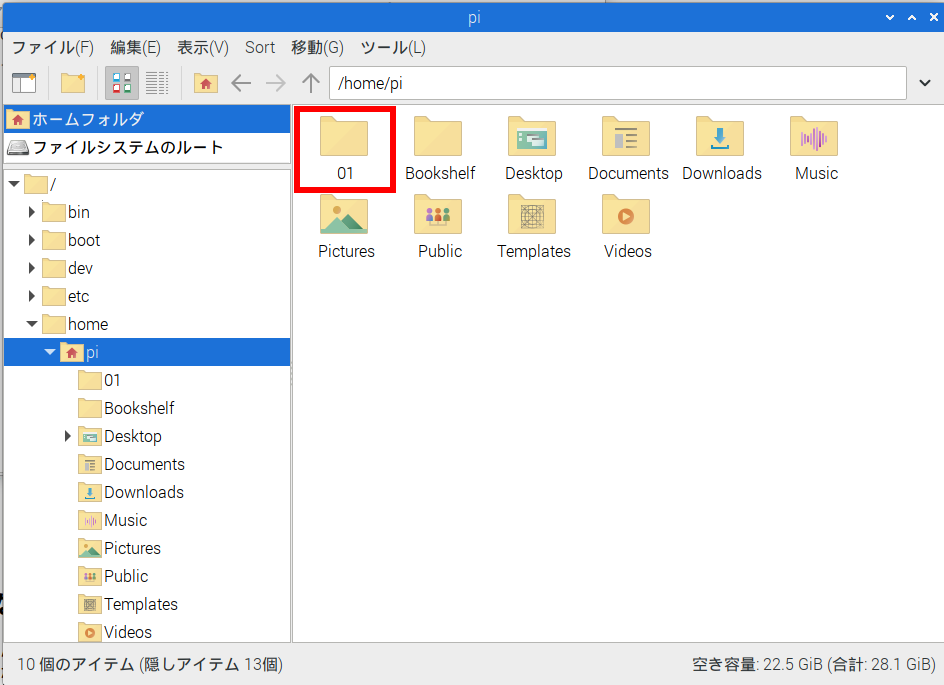
\includegraphics[width=\linewidth]{textbook-img167.png}
  \newline
  4 01をダブルクリック
\end{minipage}

\clearpage
\flushleft

\textbf{考え方}


\bigskip


\bigskip


\bigskip

\centering
\begin{minipage}{0.45\linewidth}
  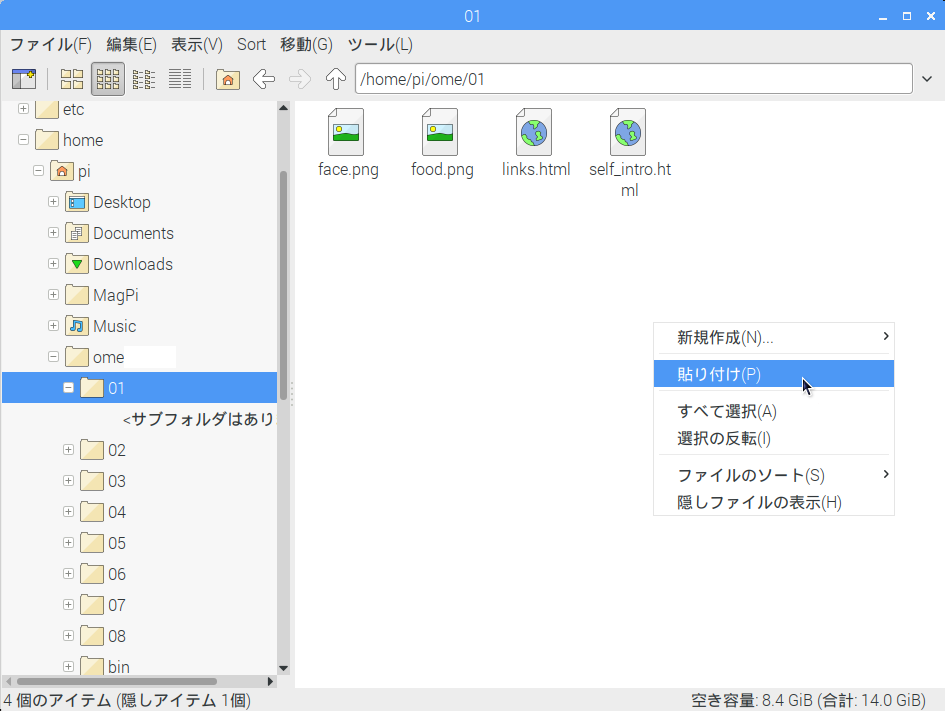
\includegraphics[width=\linewidth]{textbook-img168.png}\\
  5 右クリックして\ruby{貼}{は}り付けを\ruby{選択}{せんたく}します
\end{minipage}
\hfill
\vspace{20pt}
\begin{minipage}{0.45\linewidth}
  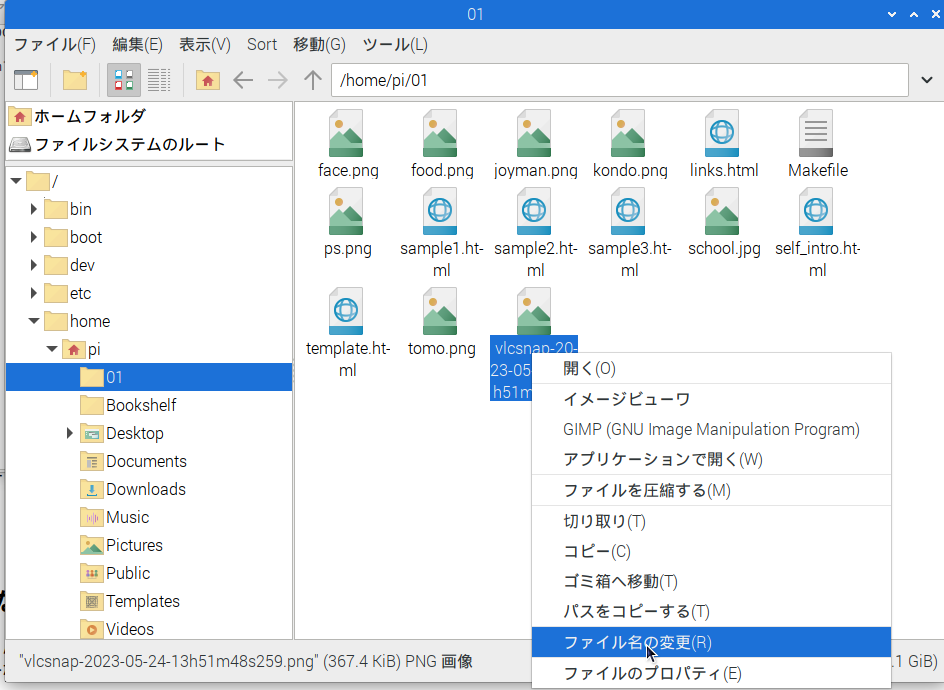
\includegraphics[width=\linewidth]{textbook-img169.png}\\
  6 \ruby{貼}{は}り付けたファイルを右クリックして、「ファイル名の\ruby{変更}{へんこう}」をします
\end{minipage}
\begin{minipage}{0.45\linewidth}
  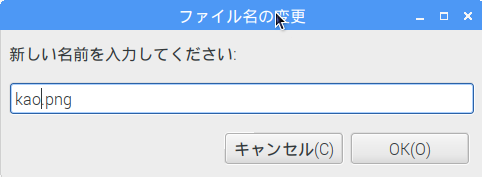
\includegraphics[width=\linewidth]{textbook-img166.png}\\
  7 今回は「kao.png」と\ruby{変更}{へんこう}します
\end{minipage}
\hfill
\vspace{20pt}
\begin{minipage}{0.45\linewidth}
  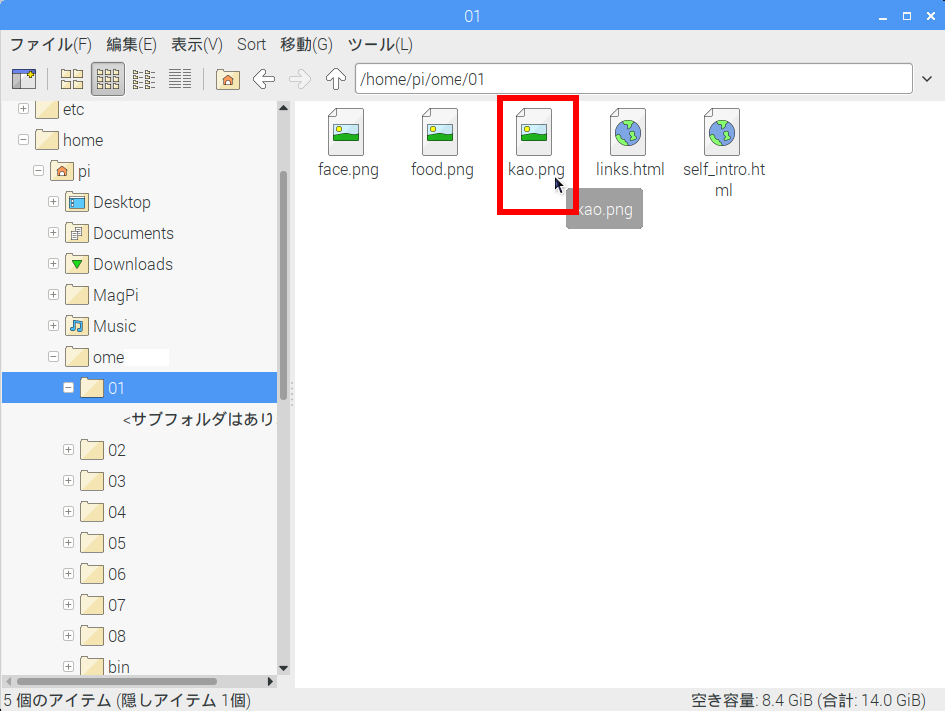
\includegraphics[width=\linewidth]{textbook-img170.png}\\
  8 これで\ruby{画像}{がぞう}のコピーは\ruby{完了}{かんりょう}です。次はhtmlを\ruby{編集}{へんしゅう}し、\ruby{自己}{じこ}\ruby{紹介}{しょうかい}ページに\ruby{表示}{ひょうじ}しましょう
\end{minipage}

\clearpage
\flushleft
\textbf{考え方}\ \


赤色で線を引いているところで\ruby{画像}{がぞう}を\ruby{表示}{ひょうじ}しています。\\
\textbf{{\textless}img href=”face.png” width=”320” height=”320”{\textgreater}}
\textbf{href=””で\ruby{画像}{がぞう}のファイルを指定しています。}\\
\textbf{“face.png”}からコピーしたファイル\textbf{(“kao.png”)}へ\ruby{変更}{へんこう}してみましょう。

\begin{minipage}{\textwidth}
  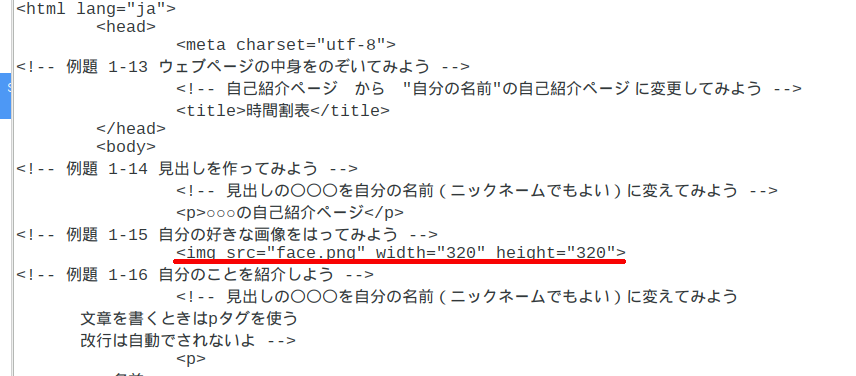
\includegraphics[width=0.6\textwidth]{textbook-img171.png}
  \newline
  \ruby{変更}{へんこう}して、\ruby{保存}{ほぞん}しリロードするととった写真が\ruby{表示}{ひょうじ}されます。
\end{minipage}

\flushleft
\textbf{答え}

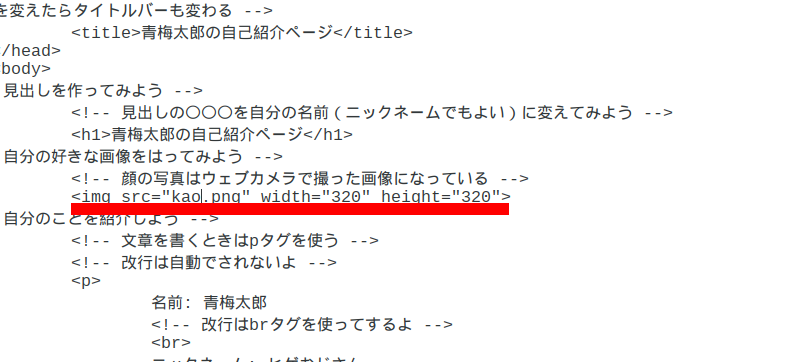
\includegraphics[width=0.6\textwidth]{textbook-img172.png}



\refstepcounter{Question}\theQuestion

スパゲッティの\ruby{画像}{がぞう}をウェブカメラでとった\ruby{画像}{がぞう}(教室の風景など)に\ruby{変更}{へんこう}しよう

ヒント

%\liststyleLxviii
\begin{enumerate}
  \item
        \ruby{画像}{がぞう}を01フォルダの中にコピーして名前を\ruby{変更}{へんこう}しよう。
  \item
        imgタグをコピーした\ruby{画像}{がぞう}を\ruby{表示}{ひょうじ}するように\ruby{変更}{へんこう}しよう
\end{enumerate}
\refstepcounter{Question}\theQuestion\label{Q:hasAnswer04-3}

width,
heightを\ruby{変更}{へんこう}して\ruby{画像}{がぞう}の大きさを変えてみましょう

ヒント

%\liststyleLxix
\begin{itemize}
  \item
        widthは横\ruby{幅}{はば}、heightはたて\ruby{幅}{はば}です。数字を変えて見ましょう。
\end{itemize}


\clearpage
\refstepcounter{Exercise}
\subsection{\theExercise 自分のことを\ruby{紹介}{しょうかい}しよう}
\addtocounter{Exercise}{-1}\refstepcounter{Exercise}\label{E:HTML_4}
\centering
\begin{minipage}{\textwidth}
  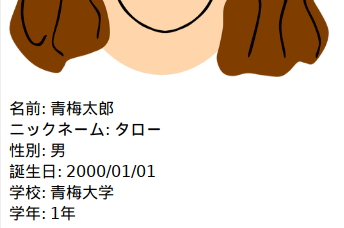
\includegraphics[width=0.5\textwidth]{textbook-img173.png}
  \newline
  \stepcounter{Figure}{\theFigure}: 自分のことを\ruby{紹介}{しょうかい}しよう
\end{minipage}

\bigskip

\flushleft

\textbf{考え方}


\bigskip

まずは今回\ruby{変更}{へんこう}する場所をブラウザで見てみましょう。

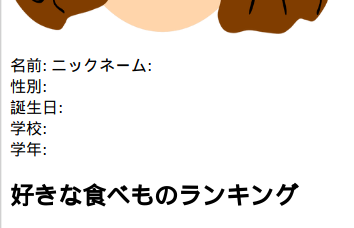
\includegraphics[width=0.5\textwidth]{textbook-img175.png}

\bigskip

\flushleft
名前とニックネームが同じ行になっていて、見づらいですね。まずは、改行の仕方を学びましょう。テキストエディタへ\ruby{戻}{もど}ってください。文章中で改行をするには\\
{\textless}br{\textgreater} \ \ \ \ \ \\
タグを使います。このタグには\ruby{終了}{しゅうりょう}タグがありません。赤線を引いてある下に{\textless}br{\textgreater}タグをいれて改行できているか確かめてみましょう。


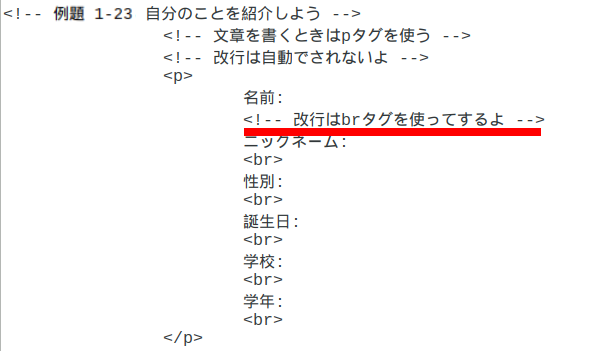
\includegraphics[width=0.5\textwidth]{textbook-img174.png}

\clearpage
\flushleft

\textbf{考え方(続き)}


これで見やすくなりましたね。

\bigskip


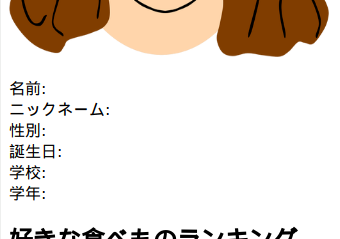
\includegraphics[width=0.5\textwidth]{textbook-img176.png}

\bigskip

次は自分のことを\ruby{紹介}{しょうかい}しよう。\\
名前、\ruby{性別}{せいべつ}、\ruby{誕生日}{たんじょうび}、学校、学年\\
を追加してみよう。



\bigskip

\bigskip


\textbf{答え}


\bigskip

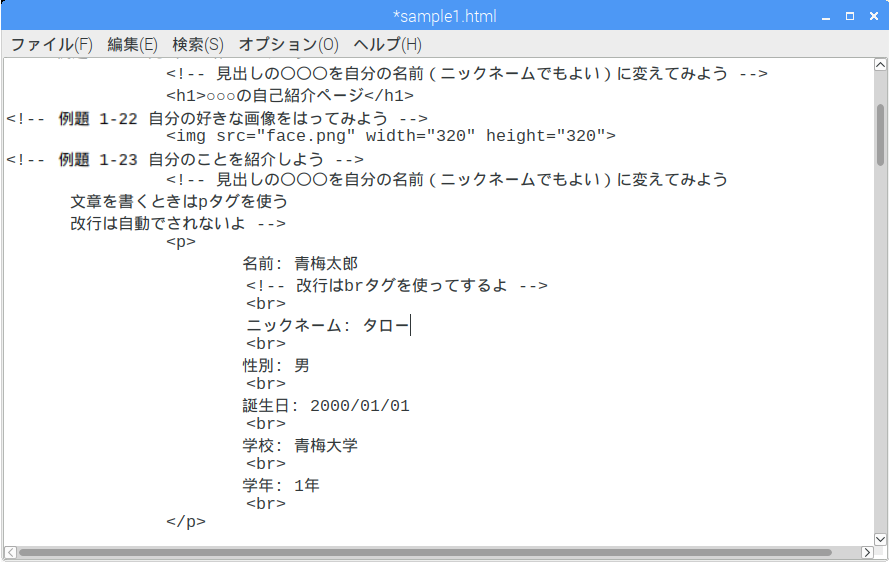
\includegraphics[width=0.5\textwidth]{textbook-img177.png}



\bigskip

\bigskip



ブラウザの画面

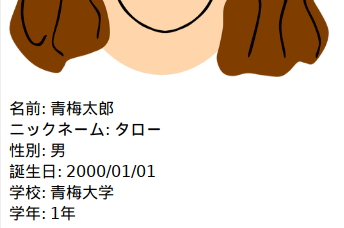
\includegraphics[width=0.5\textwidth]{textbook-img173.png}



\clearpage
\refstepcounter{Question}\theQuestion\label{Q:hasAnswer04-4}

他にも\ruby{紹介}{しょうかい}\ruby{項目}{こうもく}を追加してみましょう

%\liststyleLxx
\begin{itemize}
  \item ヒント : しゅみ、すきなもの
\end{itemize}
\refstepcounter{Question}\theQuestion\label{Q:hasAnswer04-5}

顔写真の\ruby{変更}{へんこう}

ヒント

%\liststyleLxxi
\begin{enumerate}
  \item
        01フォルダに\ruby{画像}{がぞう}をコピーしよう。
  \item とった\ruby{画像}{がぞう}はPicturesフォルダにあるよ。
  \item \ruby{画像}{がぞう}の名前を変えよう。
  \item
        imgタグを変えて、\ruby{表示}{ひょうじ}させたい\ruby{画像}{がぞう}のファイル名にしよう。
\end{enumerate}

\bigskip


\bigskip

\clearpage
\refstepcounter{Exercise}
\subsection{\theExercise ランキングを作ろう}
\addtocounter{Exercise}{-1}\refstepcounter{Exercise}\label{E:HTML_5}
自分の好きなことを\ruby{紹介}{しょうかい}するためにランキングトップ3を作ってみましょう。見出しの\ruby{変更}{へんこう}とランキングに一つ追加する必要があります。



\bigskip


\begin{minipage}{\textwidth}
  {\upshape
    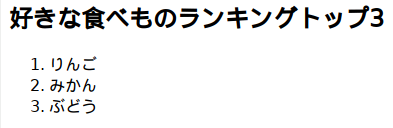
\includegraphics[width=0.65\textwidth]{textbook-img178.png}
    \newline
    \stepcounter{Figure}{\theFigure}:
    好きなたべものランキングトップ3を作ろう}
\end{minipage}


\bigskip


\bigskip

\textbf{考え方}



\bigskip



好きなたべものランキングトップ3を作ってみましょう。まずは、ブラウザで\ruby{確認}{かくにん}してみましょう。


\bigskip

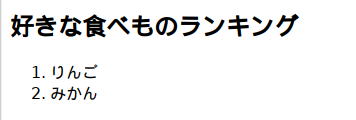
\includegraphics[width=0.65\textwidth]{textbook-img179.png}

\bigskip

まずは、見出しを\ruby{変更}{へんこう}してみましょう。\\
\textbf{好きなたべものランキングトップ3}\\
に変えてください。


\bigskip

次にランキングの作り方を説明します。\\
ランキングを作るにはリストを使います。テキストエディタを見てみましょう。

\centering
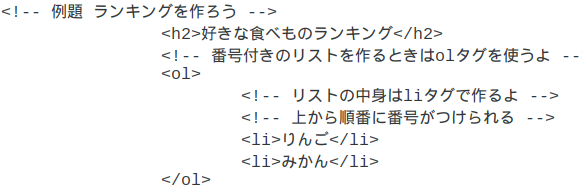
\includegraphics[width=0.6\textwidth]{textbook-img180.png}

\clearpage
\flushleft
\textbf{考え方(続き)}


\bigskip


ランキングの\textbf{りんご}は青色で線が引かれている行で\ruby{表示}{ひょうじ}をしています。


\bigskip


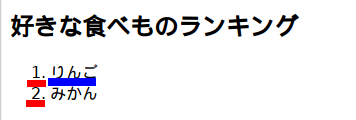
\includegraphics[width=0.65\textwidth]{textbook-img182.png}


\bigskip


%[Warning: Image ignored] % Unhandled or unsupported graphics:
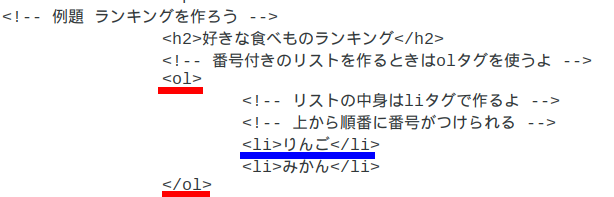
\includegraphics[width=0.6\textwidth]{textbook-img181.png}


青色で線が引かれている行の\\
{\textless}li{\textgreater}りんご{\textless}/li{\textgreater}\\
りんごを\ruby{表示}{ひょうじ}しています。\\
順位は赤で線が引かれている\\
{\textless}ol{\textgreater}\\
{\textless}/ol{\textgreater}\\
で\ruby{表示}{ひょうじ}をしています。リストを使ってランキングを作るには、\\
{\textless}ol{\textgreater}\\
\ \ {\textless}li{\textgreater}りんご{\textless}/li{\textgreater}\\
{\textless}/ol{\textgreater}\\
のように順位をつけるolタグの中でliタグを使い文字を囲みます。\\
練習として\textbf{ぶどう}をランキングの一番下に追加しましょう。\\


\bigskip


\includegraphics[width=0.9\textwidth]{textbook-img183.png}


\bigskip


\ruby{保存}{ほぞん}してブラウザをリロードすると\textbf{ぶどう}が一番下に\ruby{表示}{ひょうじ}されました。書いた順番に順位がつきます。

りんご、みかん、ぶどうを\ruby{実際}{じっさい}に好きなたべものに変えてみてください。


\bigskip
\clearpage
\textbf{答え}


\bigskip



\includegraphics[width=0.9\textwidth]{textbook-img184.png}


\bigskip


\bigskip


\bigskip


\refstepcounter{Question}\theQuestion\label{Q:hasAnswer04-6}

ランキングを追加してみましょう

ヒント

%\liststyleLxxii
\begin{itemize}
  \item
        好きなお\ruby{菓子}{かし}ランキング、好きなYouTuberランキング
\end{itemize}


\bigskip

\bigskip

\refstepcounter{Question}\theQuestion\label{Q:hasAnswer04-7}

ヒント

%\liststyleLxxiii
\begin{itemize}
  \item
        {\textless}ol{\textgreater}{\textless}/ol{\textgreater}の代わりに{\textless}ul{\textgreater}{\textless}/ul{\textgreater}を使って、どうなるか\ruby{確認}{かくにん}してみましょう
\end{itemize}



\bigskip

\clearpage
\refstepcounter{Exercise}
\subsection{\theExercise 日記を書いてみよう}
\addtocounter{Exercise}{-1}\refstepcounter{Exercise}\label{E:HTML_6}
日記を書いてみよう。教室でやっていることを\ruby{紹介}{しょうかい}してみよう。

\centering
\begin{minipage}{6.32cm}
  {\upshape
    \includegraphics[width=0.45\textwidth]{textbook-img185.png}
    \newline
    \stepcounter{Figure}{\theFigure}: 日記を書いてみよう}
\end{minipage}

\bigskip

\flushleft
\textbf{考え方}



文章を書くときは{\textless}p{\textgreater}{\textless}/p{\textgreater}を使うと習いました。

文字の太さ、色を変えたり、アンダーライン、ななめ文字にすることもできます。

\centering
\includegraphics[width=14.284cm]{textbook-img186.png}

\bigskip

\flushleft

イタリックはななめの文字です。イタリックという文字が少しななめになっているのを\ruby{確認}{かくにん}してみましょう\\
{\textless}i{\textgreater}イタリック{\textless}/i{\textgreater}\\

\bigskip

アンダーラインは文字の下に線を引きます。\\
{\textless}u{\textgreater}アンダーライン{\textless}/u{\textgreater}\\

\bigskip

太文字は文字を太くします\\
{\textless}strong{\textgreater}\textbf{あいうえお}{\textless}/strong{\textgreater}


\bigskip
色付きの文字は
\textbf{{\textless}font color=”\#RRGGBB”{\textgreater}色文字{\textless}/font{\textgreater}}
として光の三原色を用いて色を指定します。\\
\textbf{RR}は赤の強さ\\
\textbf{GG}は緑の強さ\\
\textbf{BB}は青の強さを、
それぞれ00からFFの16進数で指定します。
例えば、赤は"\#FF0000"、緑は"\#00FF00"、青は"\#0000FF"、白は"\#FFFFFF"、黒は"\#000000"

\bigskip
\textbf{16進数は、0から9の次に、A,B,C,D,E,Fを用いて、
  1\ruby{桁}{けた}を16個の\ruby{数値}{すうち}で表します。}

\bigskip



\clearpage
\textbf{考え方(続き)}



\textbf{\ruby{授業}{じゅぎょう}で使用したホームページ\url{links.html}の2番目}を開いて見てください。
2番を開くと地下鉄で使っている色の見本が出てきます。
\ruby{銀座線}{ぎんざせん}オレンジは\textbf{\#f39700}となっているので、
上のcolorの\ruby{値}{あたい}を”\#f39700”とします。
このように\ruby{数値}{すうち}によって\ruby{表示}{ひょうじ}する色を選びます。



\bigskip

\includegraphics[width=\textwidth]{textbook-img187.png}

文字の大きさを変えるときは

\textbf{{\textless}font size=”1”{\textgreater}文字の大きさ{\textless}/font{\textgreater}}

\textbf{size=”1”}で文字の大きさを変えられます。1を他の数字に変えてみてください。

このように文字のとくちょうを変えることができます。


\bigskip

これらのタグを使って日記を書いてみよう。

下の日記を参考にしてみよう


\bigskip

\includegraphics[width=8.779cm]{textbook-img185.png}

\clearpage
\textbf{答え}



\includegraphics[width=\textwidth]{textbook-img188.png}

\refstepcounter{Question}\theQuestion\label{Q:hasAnswer04-8}
\textbf{{\textless}hr{\textgreater}}タグを使うと横線を引くことができます。日記の一番下に横線を引いてみよう。

ヒント

%\liststyleLxxiv
\begin{itemize}
  \item
        \ruby{終了}{しゅうりょう}タグはhrタグにありません。{\textless}hr{\textgreater}と書いたところに横線が\ruby{表示}{ひょうじ}されます。
\end{itemize}
\refstepcounter{Question}\theQuestion\label{Q:hasAnswer04-9}

日記をもう一つ追加してみよう

ヒント

%\liststyleLxxv
\begin{itemize}
  \item
        タイトル、日付、本文を順番に書いてみよう。
\end{itemize}
\clearpage
\refstepcounter{Exercise}
\subsection{\theExercise グループのメンバー表を作ろう}
\addtocounter{Exercise}{-1}\refstepcounter{Exercise}\label{E:HTML_7}
グループの友だちのことを表にまとめてみよう。

\centering
\begin{minipage}{\textwidth}
  {\upshape
    \includegraphics[width=0.5\textwidth]{textbook-img189.png}
    \newline
    \stepcounter{Figure}{\theFigure}: グループメンバーの表}
\end{minipage}

\bigskip

\flushleft
\textbf{考え方}



表を作るには

{\textless}table{\textgreater}{\textless}/table{\textgreater}

を使います。

まずは、表に題名をつけます。captionタグを使います。

青色の線を見てください。

\textbf{{\textless}caption{\textgreater}みんなの\ruby{紹介}{しょうかい}{\textless}/caption{\textgreater}}

の行が表の題名として\ruby{表示}{ひょうじ}されています。



\bigskip

\includegraphics[width=13.462cm]{textbook-img190.png}


\bigskip

その次に、列の見出しをつけます。緑色で囲われているところを見てください。\\
表の1行目に名前、学校、学年という\ruby{項目}{こうもく}があります。行は横方向です。\\
行を作るにはtrタグを使います。\\
行の見出しはthタグを使います。\\


\bigskip

{\textless}tr{\textgreater}\\
\ \ {\textless}th{\textgreater}名前{\textless}/th{\textgreater}\\
{\textless}/tr{\textgreater}\\

\bigskip

\clearpage
\textbf{考え方(続き)}



\bigskip

\bigskip


\centering
\includegraphics[width=\textwidth]{textbook-img191.png}

\flushleft

\bigskip

表の1行目にある見出しの次は\ruby{実際}{じっさい}の\ruby{情報}{じょうほう}がきます。2行目は青色で囲われているところです。

0くんのことが書いてあります。行を作るにはtrタグを使います。

見出しではthタグを使いました。見出しでない行ではtdタグを使って列の\ruby{情報}{じょうほう}を\ruby{表示}{ひょうじ}させます。

{\textless}tr{\textgreater}

\ \ {\textless}td{\textgreater}0くん{\textless}/td{\textgreater}

\ \ {\textless}td{\textgreater}c中学校{\textless}/td{\textgreater}

\ \ {\textless}td{\textgreater}2年生{\textless}/td{\textgreater}

{\textless}/tr{\textgreater}

一個目のtdタグは一個目のthタグに\ruby{対応}{たいおう}しています。つまり、一個目のthタグの\textbf{名前}は一個目のtdタグの0くんに\ruby{対応}{たいおう}しています。


\bigskip


\bigskip

グループのメンバーの友だちの名前、学校、学年を聞いてtdタグを書き\ruby{換}{か}えてみよう。


\bigskip


\bigskip



\bigskip

\clearpage
\textbf{答え}




\bigskip


\bigskip


\bigskip
\includegraphics[width=\textwidth]{textbook-img192.png}




\bigskip

\bigskip

\bigskip

\refstepcounter{Question}\theQuestion

表にクラスを追加してみよう。

ヒント

%\liststyleLxxvi
\begin{enumerate}
  \item クラスを見出しに追加してみよう
  \item
        みんなのクラスを聞いて、追加してみよう
\end{enumerate}
\refstepcounter{Question}\theQuestion

TAのことを追加してみよう

%\liststyleLxxvii
\begin{itemize}
  \item
        TAの先生に名前、学校、学年、クラスを聞いて表に追加してみよう
\end{itemize}

\bigskip

\clearpage

\refstepcounter{Exercise}
\subsection{\theExercise 自分の好きなホームページを\ruby{紹介}{しょうかい}しよう}
\addtocounter{Exercise}{-1}\refstepcounter{Exercise}\label{E:HTML_8}
自分のお気に入りのサイトを自分のホームページで\ruby{紹介}{しょうかい}しよう。



\centering
\begin{minipage}{\textwidth}
  {\upshape
    \centering
    \includegraphics[width=0.4\textwidth]{textbook-img193.png}
    \newline
    \stepcounter{Figure}{\theFigure}:
    自分の好きなホームページを\ruby{紹介}{しょうかい}しよう}
\end{minipage}



\bigskip

\flushleft

\textbf{考え方}



まずはブラウザを見てみましょう。赤線で線を引いてあるところはリンクといい、クリックすると登録されているホームページへ\ruby{移動}{いどう}します。試しにgoogleをクリックして見てください。


\bigskip

\centering
\includegraphics[width=0.22\textwidth]{textbook-img194.png}


\flushleft

\bigskip

クリックをするとブラウザで開いているページがリンクされているページへ\ruby{移動}{いどう}します。

赤色で囲われているところがホームページの住所にあたる部分です。この部分をリンクとして登録します。青色で囲われている矢印を\ruby{押}{お}すと前のページへ\ruby{戻}{もど}ります。自分のページへ\ruby{戻}{もど}りましょう。



\bigskip

\centering
\includegraphics[width=0.22\textwidth]{textbook-img195.png}

\bigskip

\flushleft
次は、タイピングゲームをクリックして見てください。今回はページは\ruby{移動}{いどう}しません。まだタイピングゲームのホームページを登録していないからです。


\clearpage
\textbf{考え方(続き)}



試しに少し前に遊んだタイピングゲームを自分のページから\ruby{移動}{いどう}できるようにしておきましょう。まずは、タイピングゲームのページを開いてください。開けたら赤線を引いたホームページの住所にあたる部分をクリックします。その後、右クリックをして\textbf{すべてを\ruby{選択}{せんたく}(A)}をクリックします。


\bigskip

\centering
\includegraphics[width=0.3\textwidth]{textbook-img196.png}

\flushleft

その後、赤線を引いてある住所にあたる部分が青くなります。そしたらまた右クリックをして

\textbf{コピー(C)}をクリックします。住所にあたる部分をコピーしました。

\centering
\includegraphics[width=0.3\textwidth]{textbook-img197.png}

\bigskip
\flushleft

次は、テキストエディタを開きます。

\centering
\includegraphics[width=\textwidth]{textbook-img198.png}

\bigskip
\flushleft

リンクは赤線を引いてあるように

{\textless}a
href=”ホームページの住所”{\textgreater}タイピングゲーム{\textless}/a{\textgreater}

と書きます。今の\ruby{状態}{じょうたい}では\textbf{ホームページの住所}はくうらんです。

くうらんになっているところを左クリックしてから右クリックします。そこで\textbf{\ruby{貼}{は}り付け(P)}をします。





\centering
\includegraphics[width=0.25\textwidth]{textbook-img199.png}

\clearpage
\flushleft
\textbf{考え方(続き)}


\bigskip

\centering
\includegraphics[width=\textwidth]{textbook-img200.png}

\bigskip
\flushleft

これでタイピングゲームのホームページの住所を登録できました。\ruby{保存}{ほぞん}してブラウザをリロードしてください。タイピングゲームをクリックするとタイピングゲームのホームページへ\ruby{移動}{いどう}するようになりました。


\bigskip
\centering
\includegraphics[width=0.25\textwidth]{textbook-img201.png}


\flushleft
このようにリンクを追加します。自分の好きなホームページをリンクとして\ruby{表示}{ひょうじ}してみてください。

ちなみに、\ruby{先程}{さきほど}のランキングを作るときにはolタグを使って\ruby{順序}{じゅんじょ}をつけました。今回は\ruby{順序}{じゅんじょ}ではなく${\bullet}を使っています。そのため青線で引いたように${\textless}ul{\textgreater}{\textless}/ul{\textgreater}を代わりに使います。

ulタグをolタグに変えれば\ruby{順序}{じゅんじょ}をつけることができます。


\bigskip

\textbf{答え}

\centering
\includegraphics[width=0.9\textwidth]{textbook-img202.png}

\flushleft
\refstepcounter{Question}\theQuestion\label{Q:hasAnswer04-10}


ホームページのランキングを作ってみよう。

ヒント

%\liststyleLxxviii
\begin{enumerate}
  \item リストに\ruby{順序}{じゅんじょ}をつけよう
  \item リストの\ruby{項目}{こうもく}をaタグにしよう
\end{enumerate}

\clearpage
\refstepcounter{Exercise}
\subsection{\theExercise 教室の使うものリストを作ろう}
教室に使うものリストを作ろう

\bigskip
\centering
\begin{minipage}{5.937cm}
  {\upshape
    \includegraphics[width=5.937cm]{textbook-img203.png}
    \newline
    \stepcounter{Figure}{\theFigure}: 教室で使うものリスト}
\end{minipage}

\bigskip
\flushleft

\textbf{考え方}



リストを作るのには

{\textless}ul{\textgreater}

\ \ {\textless}li{\textgreater}リスト\ruby{項目}{こうもく}1{\textless}/li{\textgreater}

{\textless}/ul{\textgreater}

のように書くと習いました。リストの中にリストを入れることもできます。

テキストエディタを見てください

\bigskip

\centering
\includegraphics[width=0.9\textwidth]{textbook-img204.png}

\bigskip
\flushleft

赤線が引かれているulタグの中に青色で囲われているulタグがありますね。ブラウザで見てみると、

${\bullet}持ち帰るもの$

\ \ ◯ラズベリーパイ

のようになっています。このように、ulタグの中でulタグを使うと、リストの中でリストをかけるようになります。

ラズベリーパイの下に\ruby{項目}{こうもく}を追加してみましょう。


\bigskip


\clearpage\flushleft
\textbf{答え}


\bigskip

\centering
\begin{minipage}{0.45\linewidth}
  \includegraphics[width=\linewidth]{textbook-img1043.png}
\end{minipage}
\hfill
\vspace{20pt}
\begin{minipage}{0.45\linewidth}
  \includegraphics[width=\linewidth]{textbook-img1044.png}
\end{minipage}

\bigskip
\flushleft

\refstepcounter{Question}\theQuestion\label{Q:hasAnswer04-11}

持ち物の\ruby{画像}{がぞう}をとって、\ruby{項目}{こうもく}の下に\ruby{貼}{は}ろう

ヒント

%\liststyleLxxix
\begin{enumerate}
  \item
        ウェブカメラで持ち物の\ruby{画像}{がぞう}をとってみよう
  \item
        01フォルダの中に\ruby{画像}{がぞう}をコピーしよう
  \item \ruby{画像}{がぞう}の名前を\ruby{変更}{へんこう}しよう
  \item
        imgタグをliタグの下に追加して、\ruby{画像}{がぞう}を\ruby{表示}{ひょうじ}させよう。
\end{enumerate}

\bigskip


\clearpage
\end{document}
